%%%
%
% $Autor: Wings $
% $Datum: 2021-05-14 $
% $Pfad: GitLab/CornerBlending $
% $Dateiname: FirstChapter
% $Version: 4620 $
%
% !TeX spellcheck = de_DE/GB
%
%%%
\chapter{Software}

\section{Arduino IDE on PC}

\subsection{Installation}

Arduino Nano 33 BLE Sense can provide an energy-efficient and cost-effective solution for manufacturers who want to use Bluetooth Low Energy connectivity in their projects.\\

Arduino Nano 33 BLE Sense uses the Arduino software integrated development environment (IDE) for programming, which is the most widely used and common (IDE) for all arduino boards that can be run online and offline. This is a open-source Arduino Software (IDE) makes it easy to write code and upload it to the board. There are various version of software which is supported for each operating system (OS) e.g: mac, linux, and windows. Arduino community also provide us to start coding online and save our sketches in the cloud, this online arduino editor is most up-to-date version of the IDE includes all libraries and also supports new Arduino boards. For getting access to these software packages go to the following link \url{https://www.arduino.cc/en/software}  and get more up to date information, as there are frequent updates. These software can be used with any Arduino board, the most recent offline arduino IDE 2.0.3 can be seen in Figure, \ref{fig:arduino-creat-agent-installieren} it is also supportive for all operating systems.

\begin{figure}[h]
	\centering
	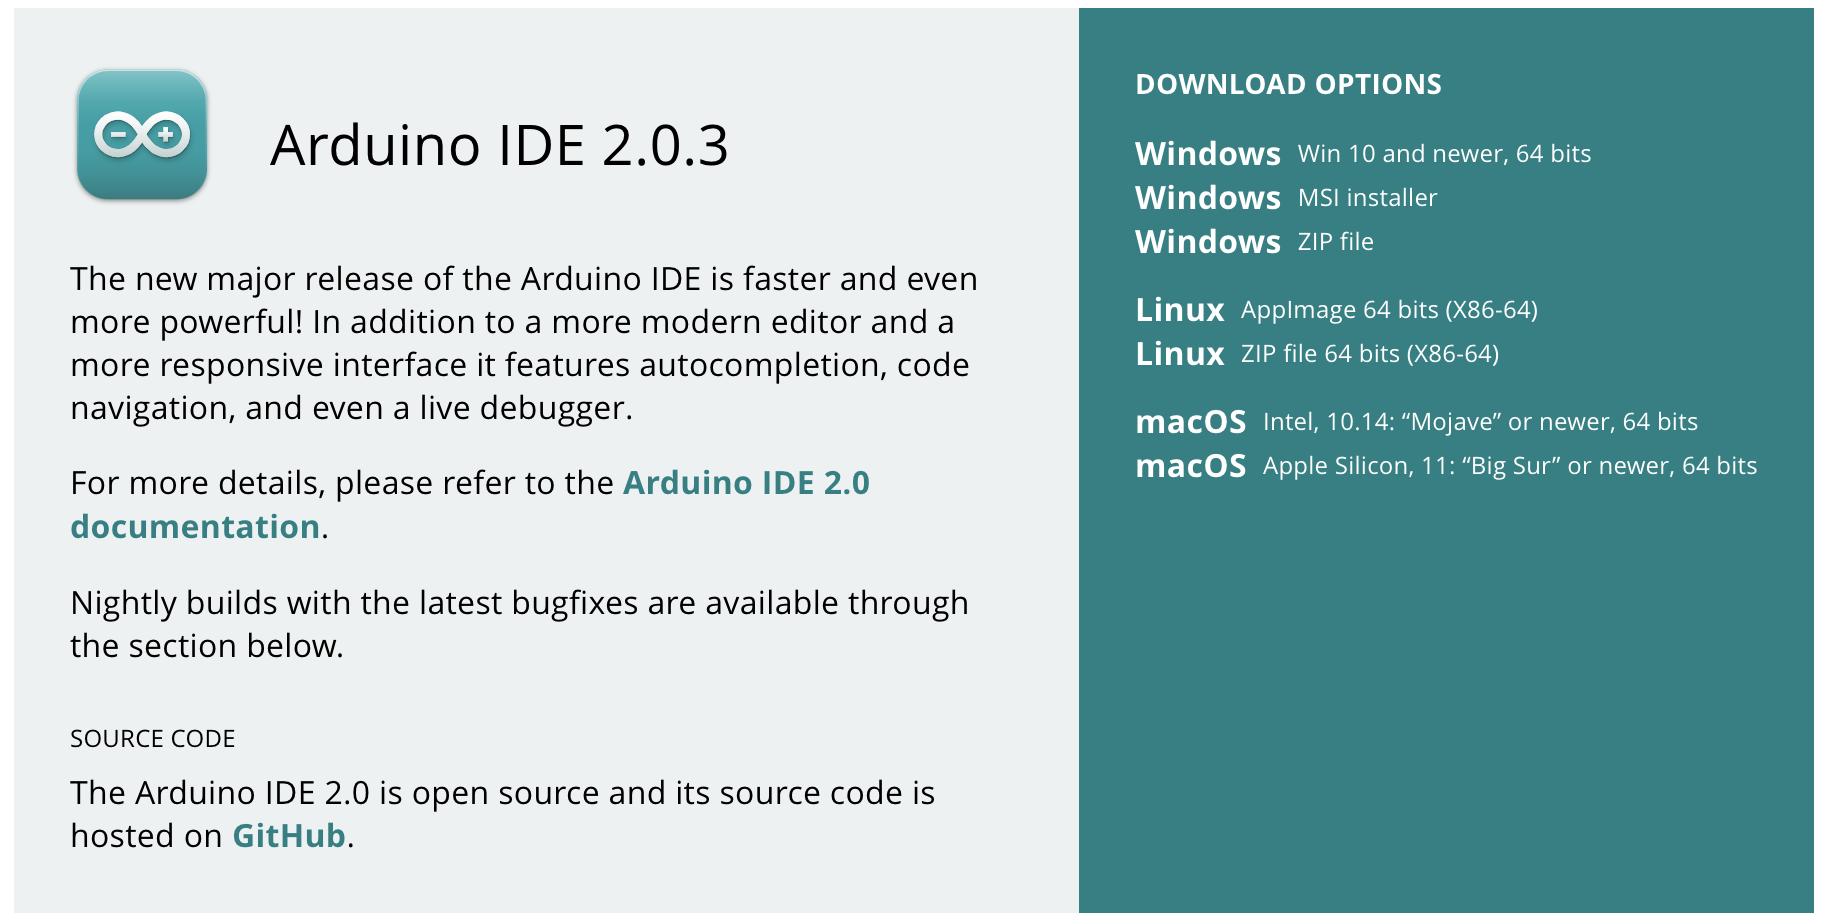
\includegraphics[width=1.0\linewidth]{Images/Arduino/Installation-1}
	\caption{Arduino Creat Agent Installation}
	\label{fig:arduino-creat-agent-installieren}
\end{figure}


\subsection{Configuration}

To program the Arduino Nano 33 BLE Sense in offline state, we need to install one of the latest arduino IDE on our desktop. After installation, for getting access to the Arduino nano 33 ble sense board, we need to make configuration in our IDE. By opening the IDE, go to tool which can be seen on the uper left corner in IDE, in the tool there is an option for managed board. At this point we need to write our board name in the search which is Arduino Nano 33 BLE Sense as shown in figure, \ref {fig:Arduino-Mbed-Boards Installation} select the Arduino Mbed OS Boards and install it. The Mbed OS nano board supports also other nano family boards including Arduino nano 33 ble sense, after installing simply connect the Arduino Nano 33 BLE Sense to the computer via USB cable. 

\begin{figure}[h]
	\centering
	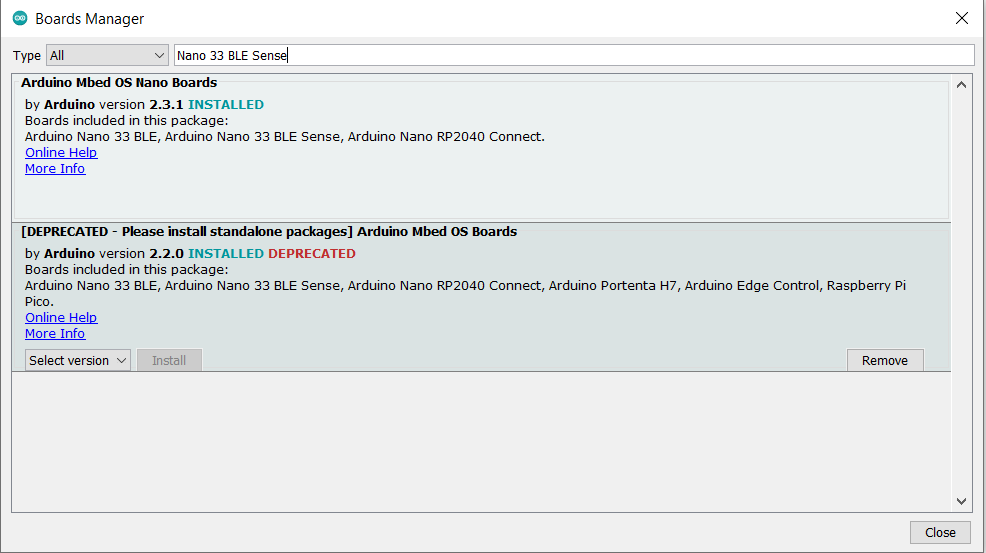
\includegraphics[width=1.0\linewidth]{Images/Nano33BLESense/Nano Mbed}
	\caption{Arduino Mbed OS Nano Boards Installation}
	\label{fig:Arduino-Mbed-Boards Installation}
\end{figure}


\subsection{Test Example}

There are set of examples which are build in Arduino (IDE) for the testing purpose, for checking all the configuration and setting up the board we can open one of the basic LED blink example first as shown in the figure.  \ref{fig:LED-Example}.

\begin{figure}[h]
	\centering
	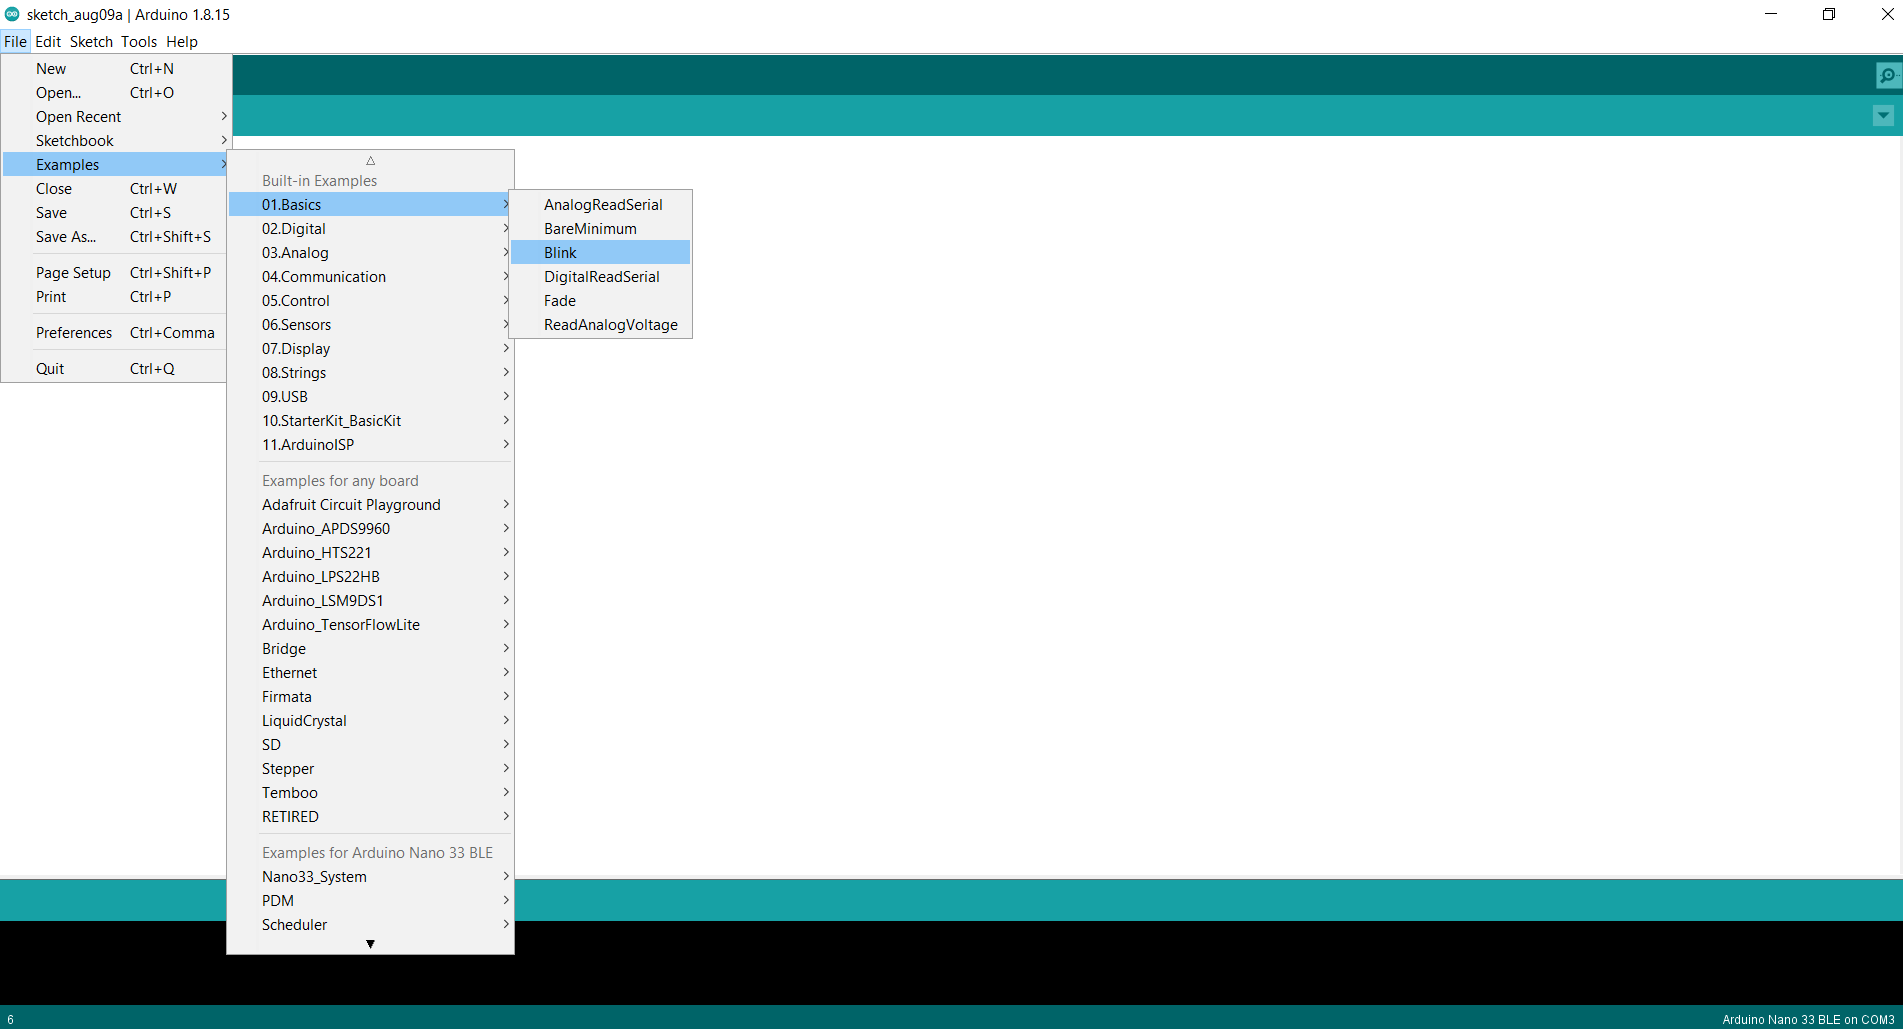
\includegraphics[width=1.0\linewidth]{Images/Arduino/LED}
	\caption{LED-Example Test}
	\label{fig:LED-Example}
\end{figure}

This LED-blink example support all the arduino boards, for the checking purposes just need to run this basic example on any arduino embed board and it will blink the LED on our Arduino board after pre-set miliseconds. In the same example folder, there are also number of build in usefull example written in Arduino IDE for embedded boards. These examples are very usefull for getting the basic knowledge about the board and programming.

\section{Pre-requisite settings for Uploading the program}

There are some pre-requisite steps need to follow either we need to run the build in example or run by our own written program. in order to program an Arduino board with a Laptop with the help of USB connection, open the Arduino IDE on desktop, a blank arduino environment page with just a Void setup and void loop written on it will appear. At this step we need to go to the tool-Arduino board and select the connected board which is Arduino Nano 33 Ble Sense as shown in the figure \ref{fig:Check Board}

\begin{figure}[h]
	\centering
	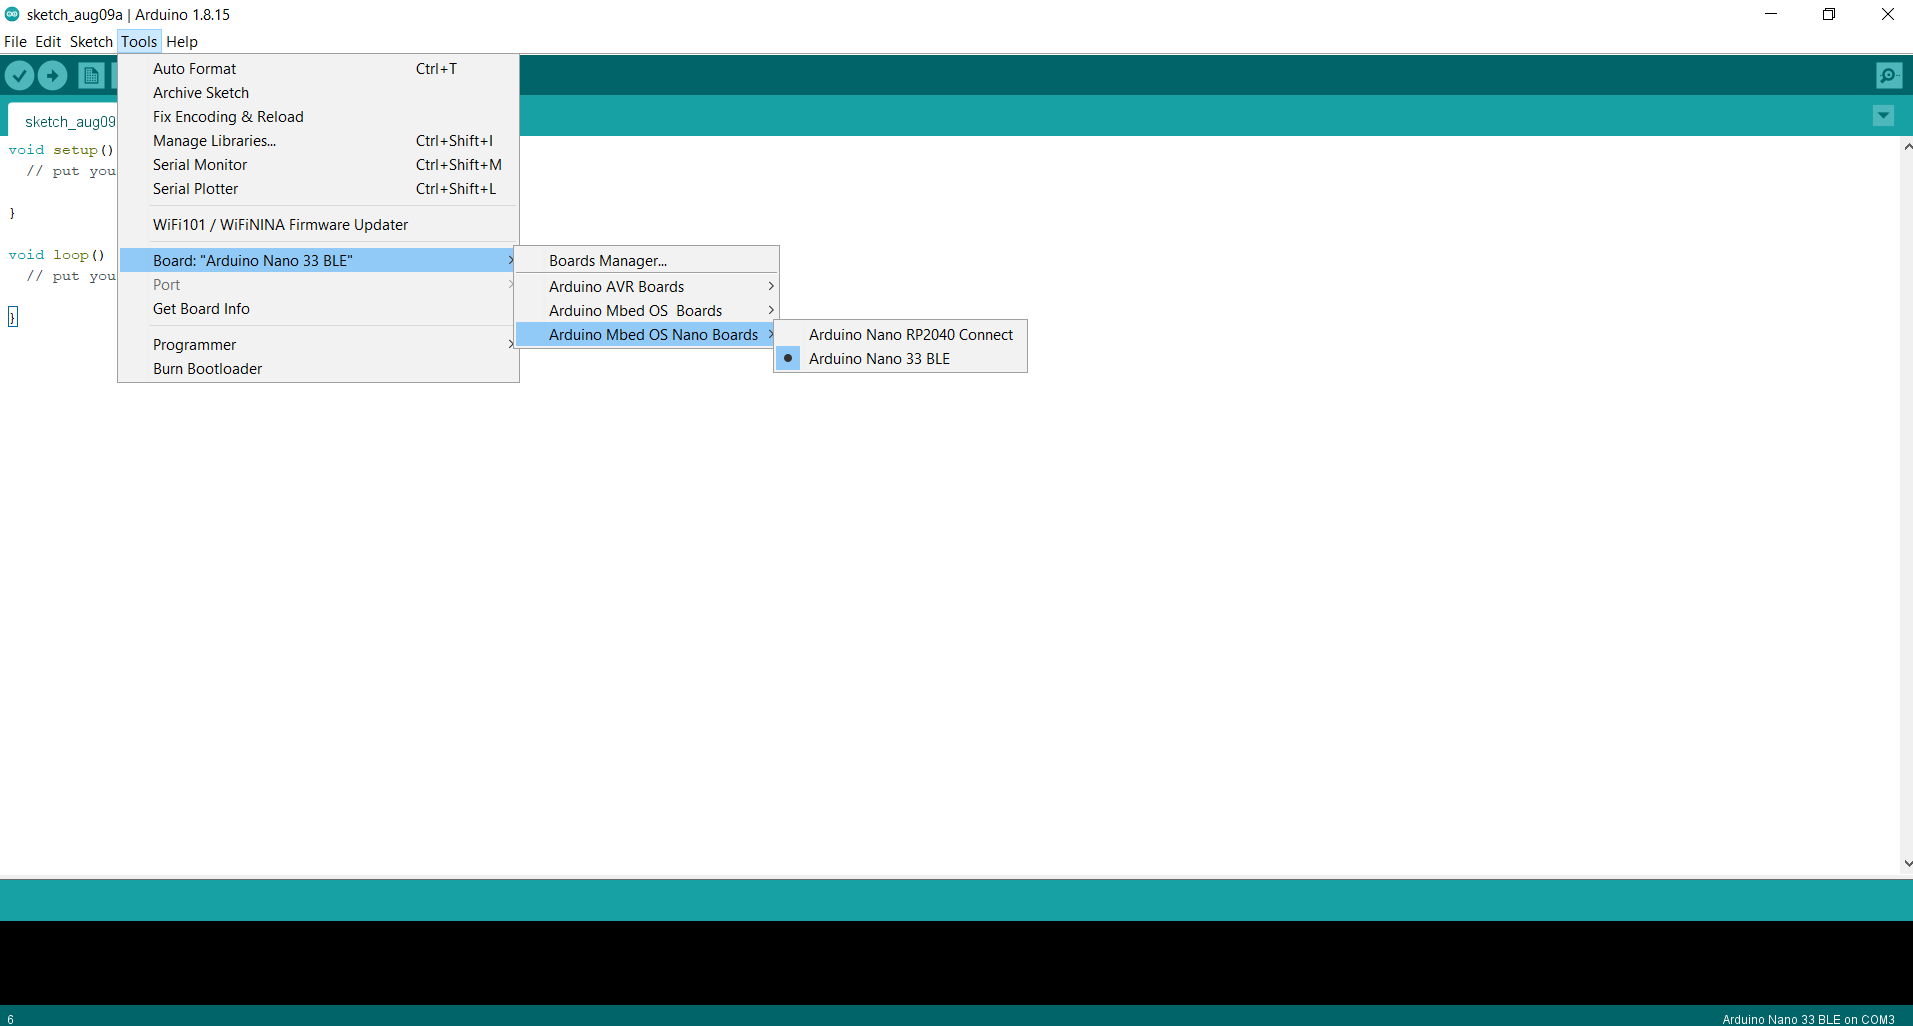
\includegraphics[width=1.0\linewidth]{Images/Arduino/Check-board}
	\caption{Select the Connected board}
	\label{fig:Check Board}
\end{figure}

\subsection{Select the Appropriate Port}

After selecting the Arduino nano 33 BLE sense board, next we need to check the connected port. For doing this, we need to set our arduino borad in Boot setup by clicking the white reset button on arduino as show in figure\ref{fig:Check-Reset}.

\begin{figure}[h]
	\centering
	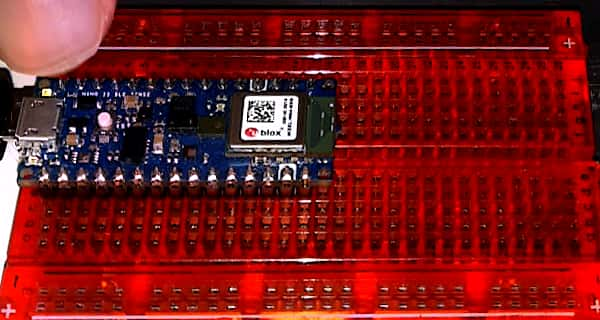
\includegraphics[width=1.0\linewidth]{Images/Arduino/Click-Reset}
	\caption{Reset Button}
	\label{fig:Check-Reset}
\end{figure}

By clicking the white reset button, the arduino borad will be in boot setup and make sure to check the orange LED glow as shown in the figure \ref{fig:LED-Glow}.

\begin{figure}[h]
	\centering
	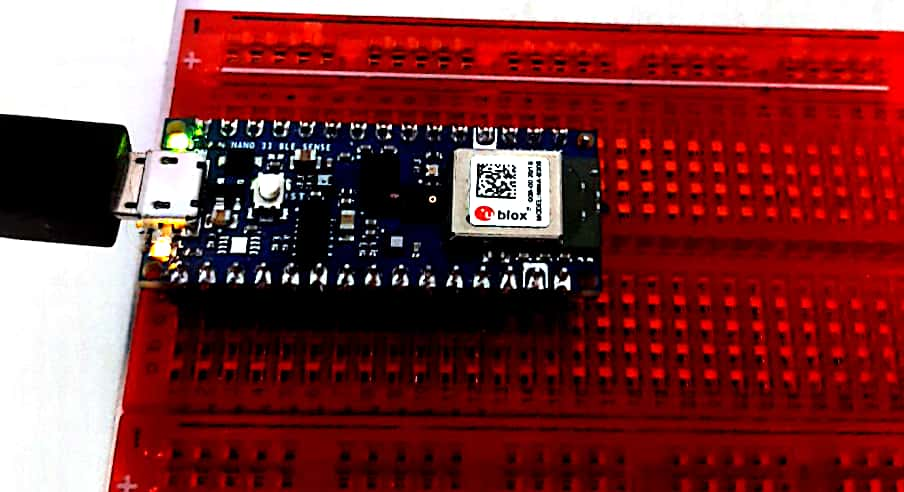
\includegraphics[width=1.0\linewidth]{Images/Nano33BLESense/Orange LED}
	\caption{Orange LED Glow}
	\label{fig:LED-Glow}
\end{figure}

After successfully applying the above mention step, next we need to select the connected port before upload the program. For this, go to tool select arduino port and make sure to check it available port for uploading the program as shown in figure \ref{fig:Port-Selection}

\begin{figure}[h]
	\centering
	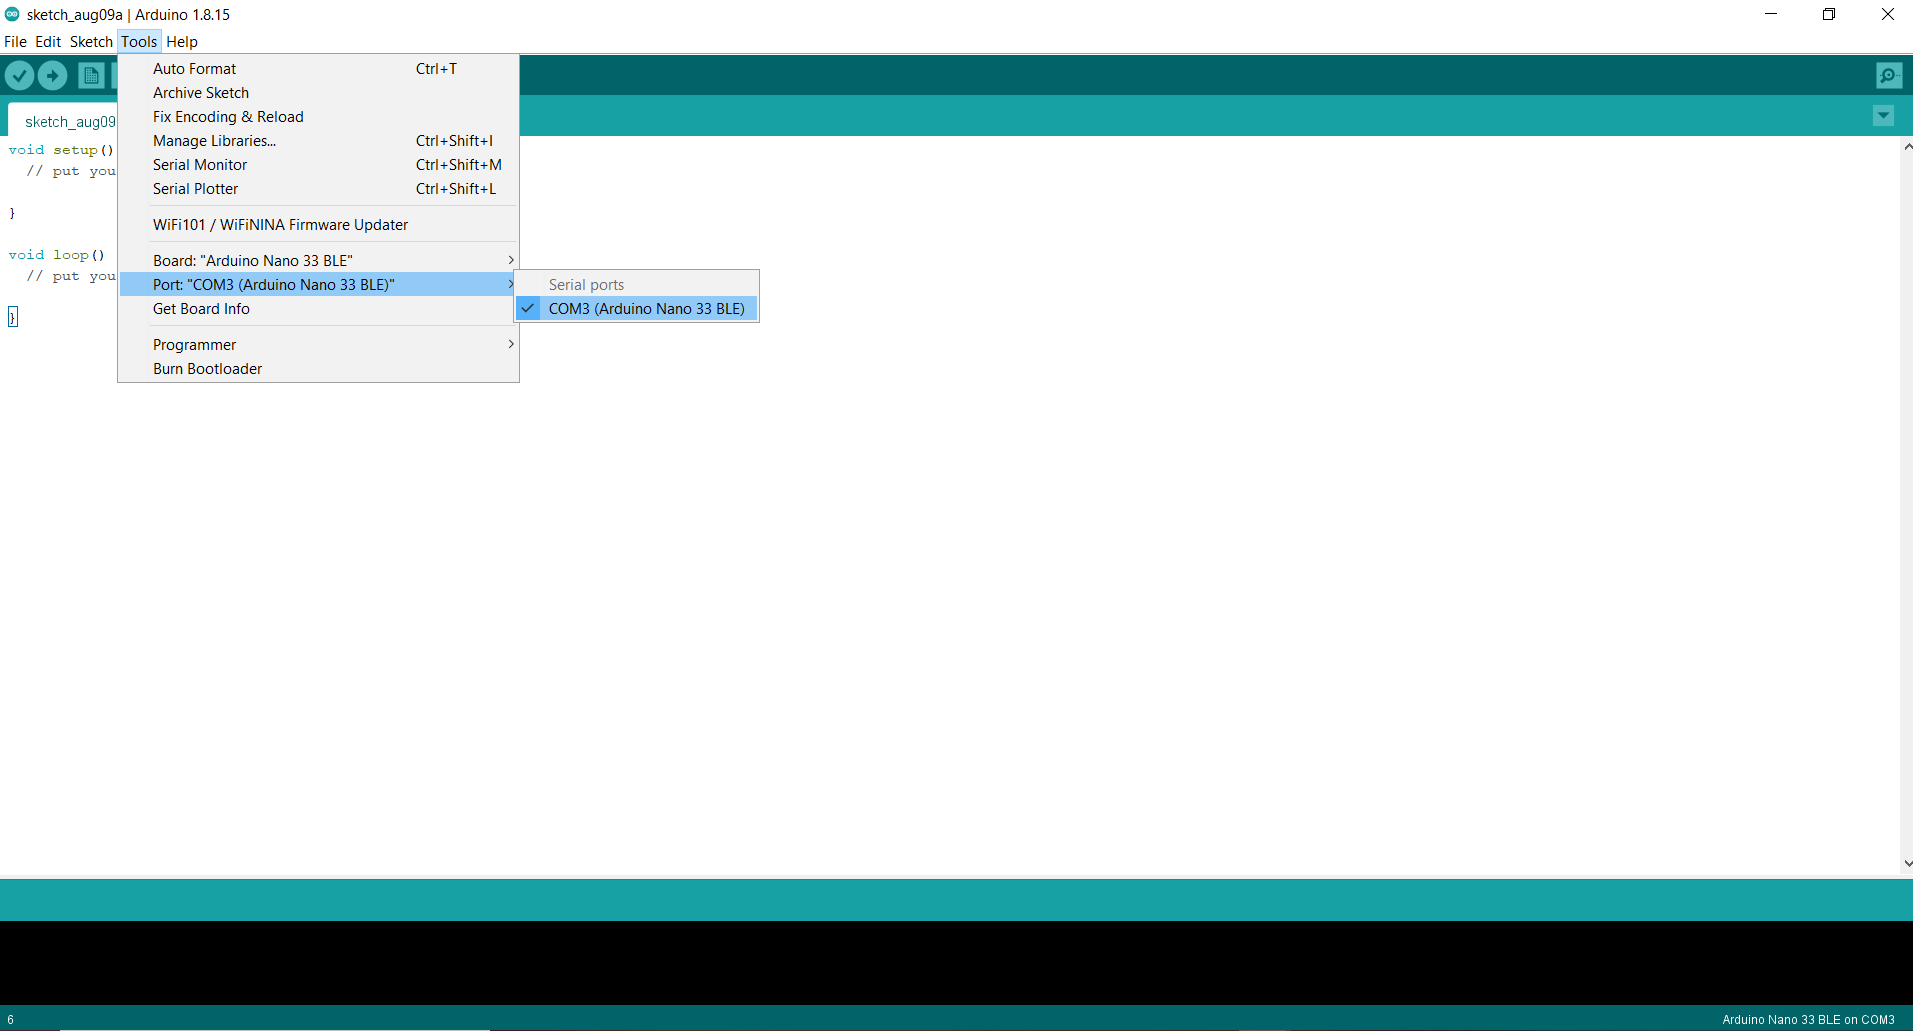
\includegraphics[width=1.0\linewidth]{Images/Arduino/Port-Select}
	\caption{Select Available Port for Uploading Arduino Sketch}
	\label{fig:Port-Selection}
\end{figure}

\subsection{Upload Code in Arduino Board}

After selecting the appropriate port, it's time to upload the Arduino program. There are five icons (verify, upload, new, open, save) below the file section, before uploading the program the best practice is to verify the program first, it show us if there are any error or warning in the program exist or not. By successfully verifying the program we can safely upload the program by click the upload button in the top below the file section as shown in figure. \ref{fig:Upload}.


\begin{figure}[h]
	\centering
	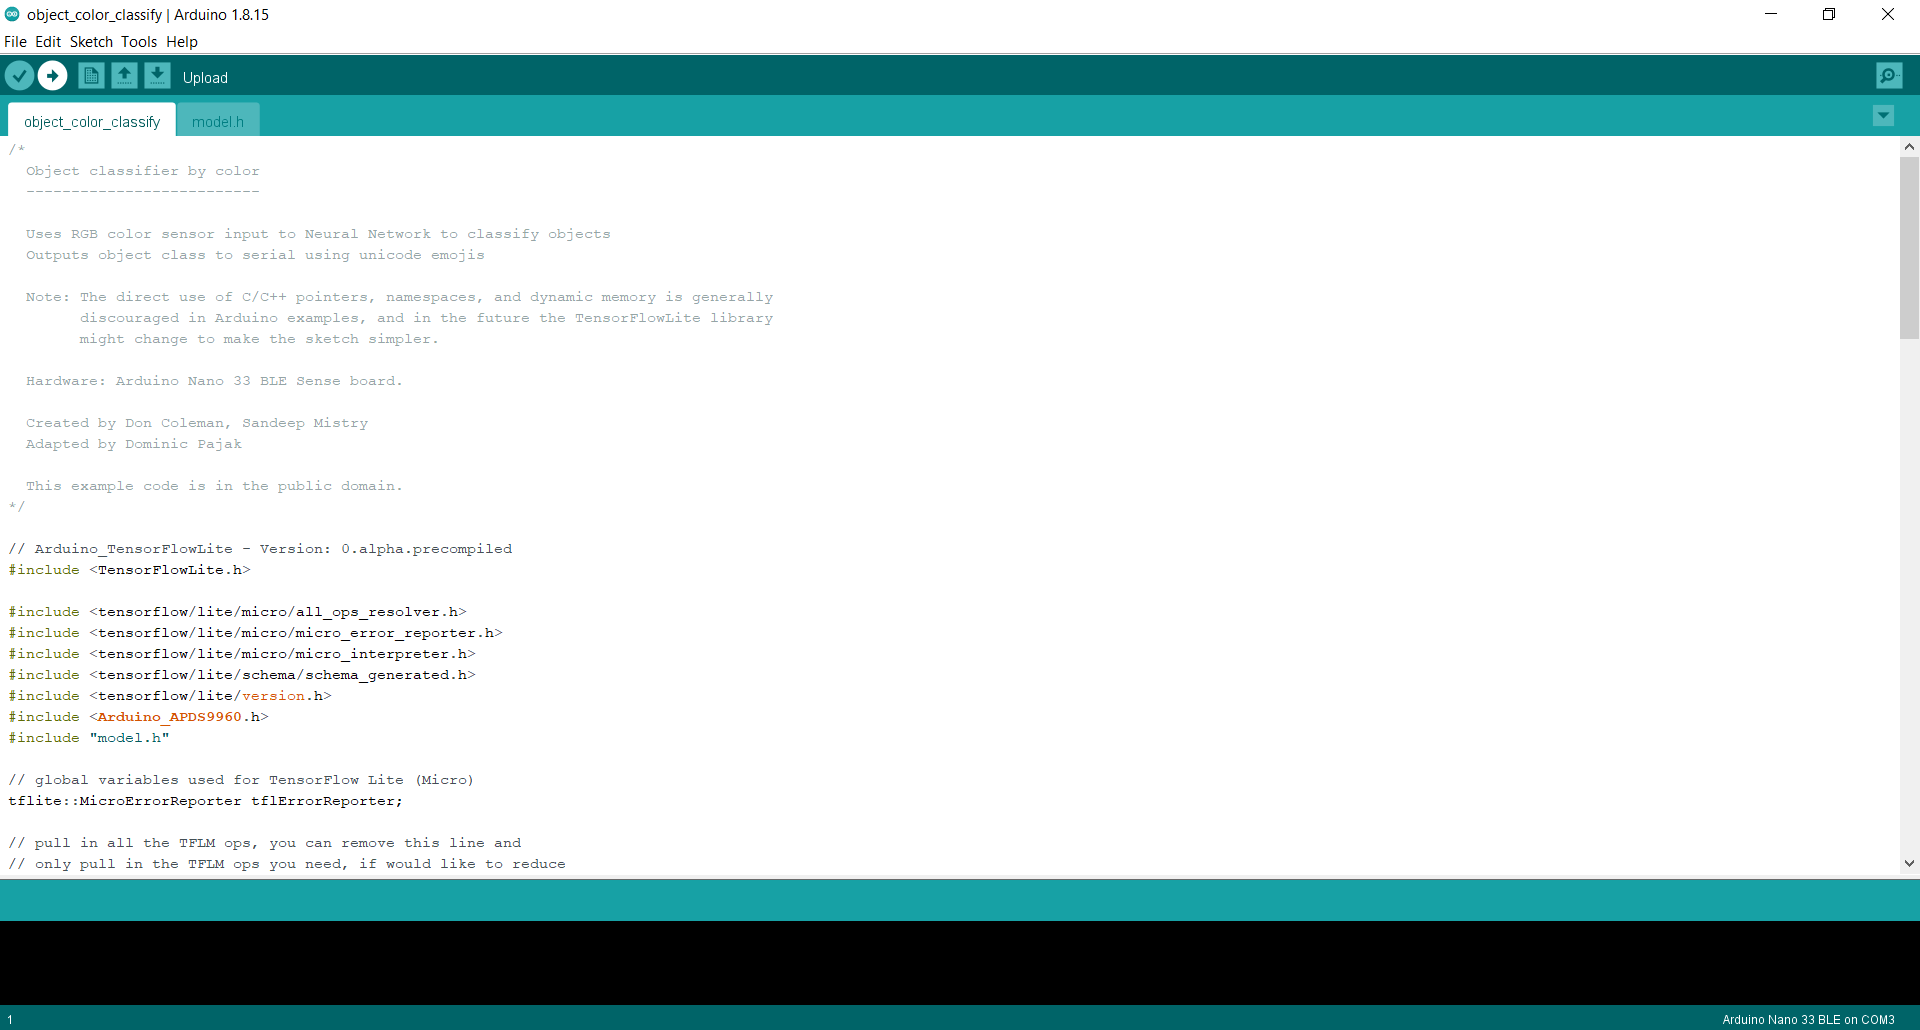
\includegraphics[width=1.0\linewidth]{Images/Arduino/Upload}
	\caption{Upload the Program in Arduino board}
	\label{fig:Upload}
\end{figure}

After uploading, the code will compile and if there is any issue in our program it will pop up in the bottom black window as well.

After successfully uploading and compiling the code in Arduino board, it also require to change the port again as we did it previously. Go to tool select arduino port and make sure to check the port again as shown in figure \ref{fig:Port} by getting output in the serial monitor.

\begin{figure}[h]
	\centering
	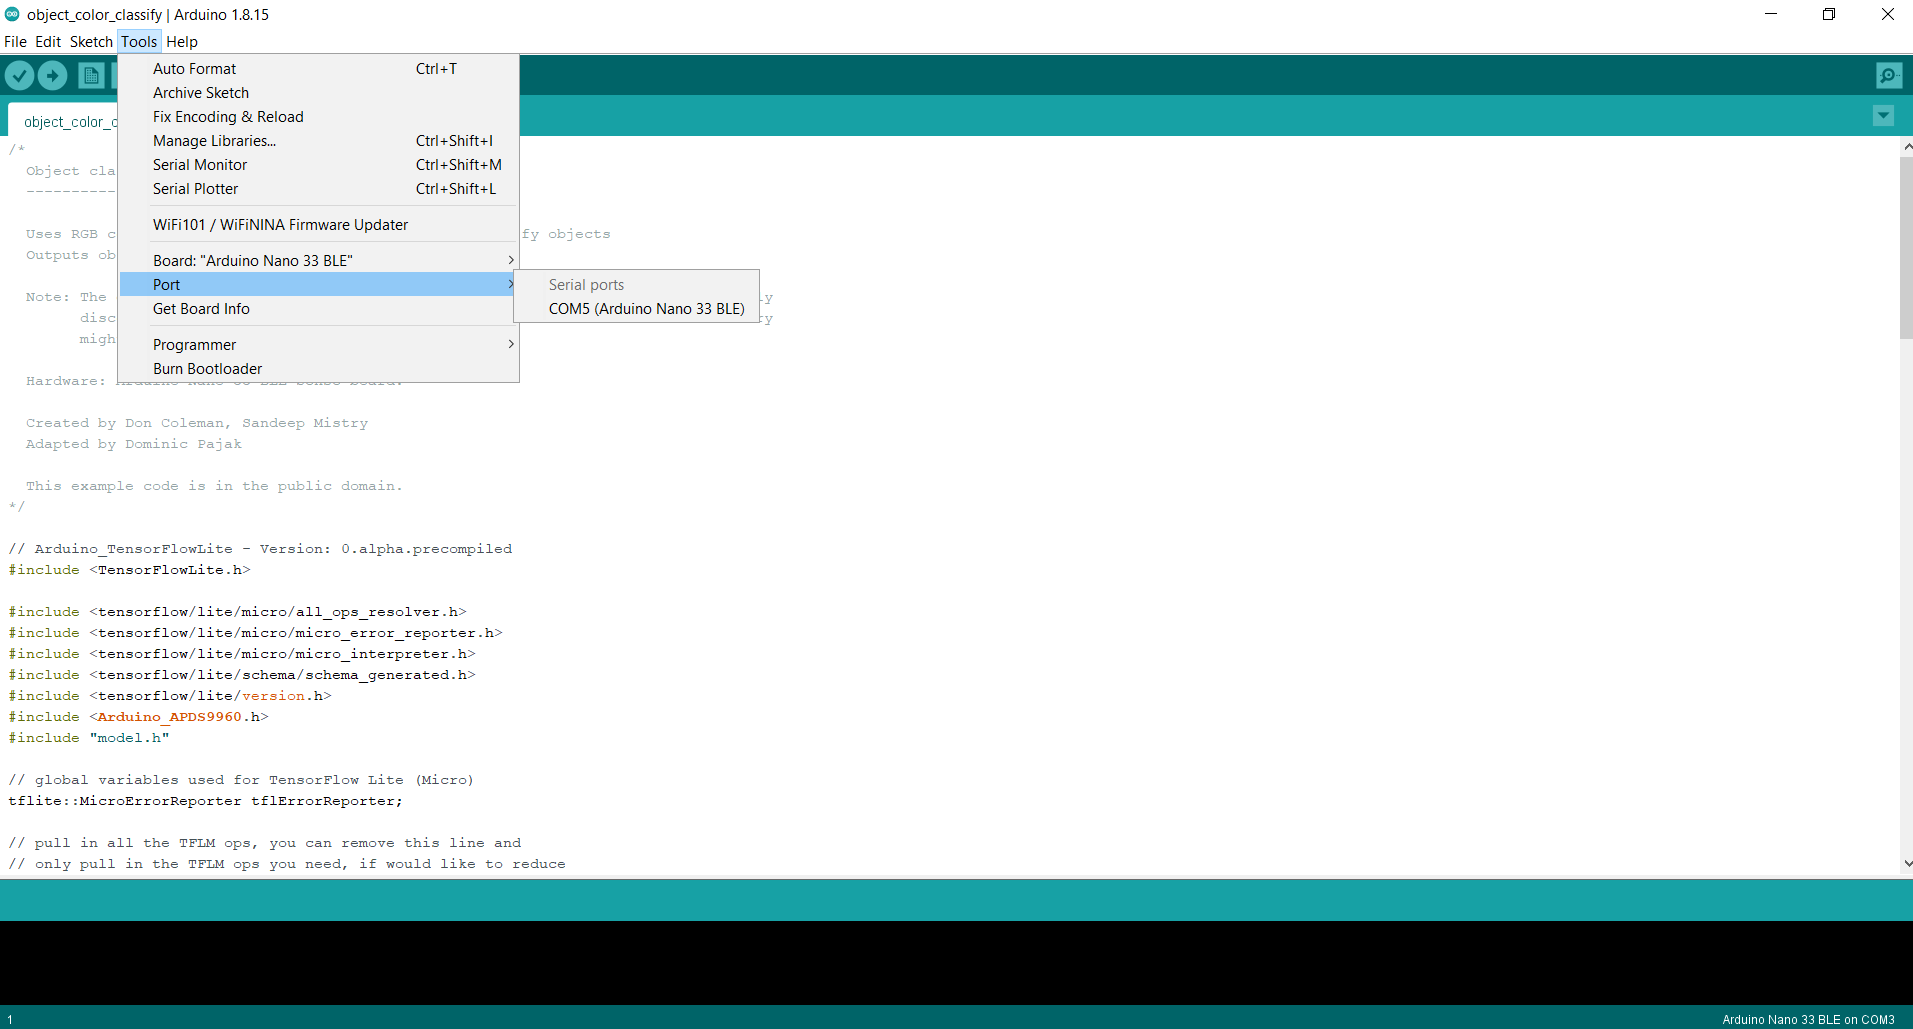
\includegraphics[width=1.0\linewidth]{Images/Arduino/Port}
	\caption{Setting the Port}
	\label{fig:Port}
\end{figure}

\section{Output Window (Serial Monitor)}

Serial Monitor is the another window on the Arduino IDE, which shows the Input/Output of our program and results appear on it as per the required output. For getting access to Serial monitor, we need to go extreme right in the Arduino IDE, the small circle pop up when we reach it is the serial monitor as show in the figure. \ref{fig:Serial Monitor}

\begin{figure}[h]
	\centering
	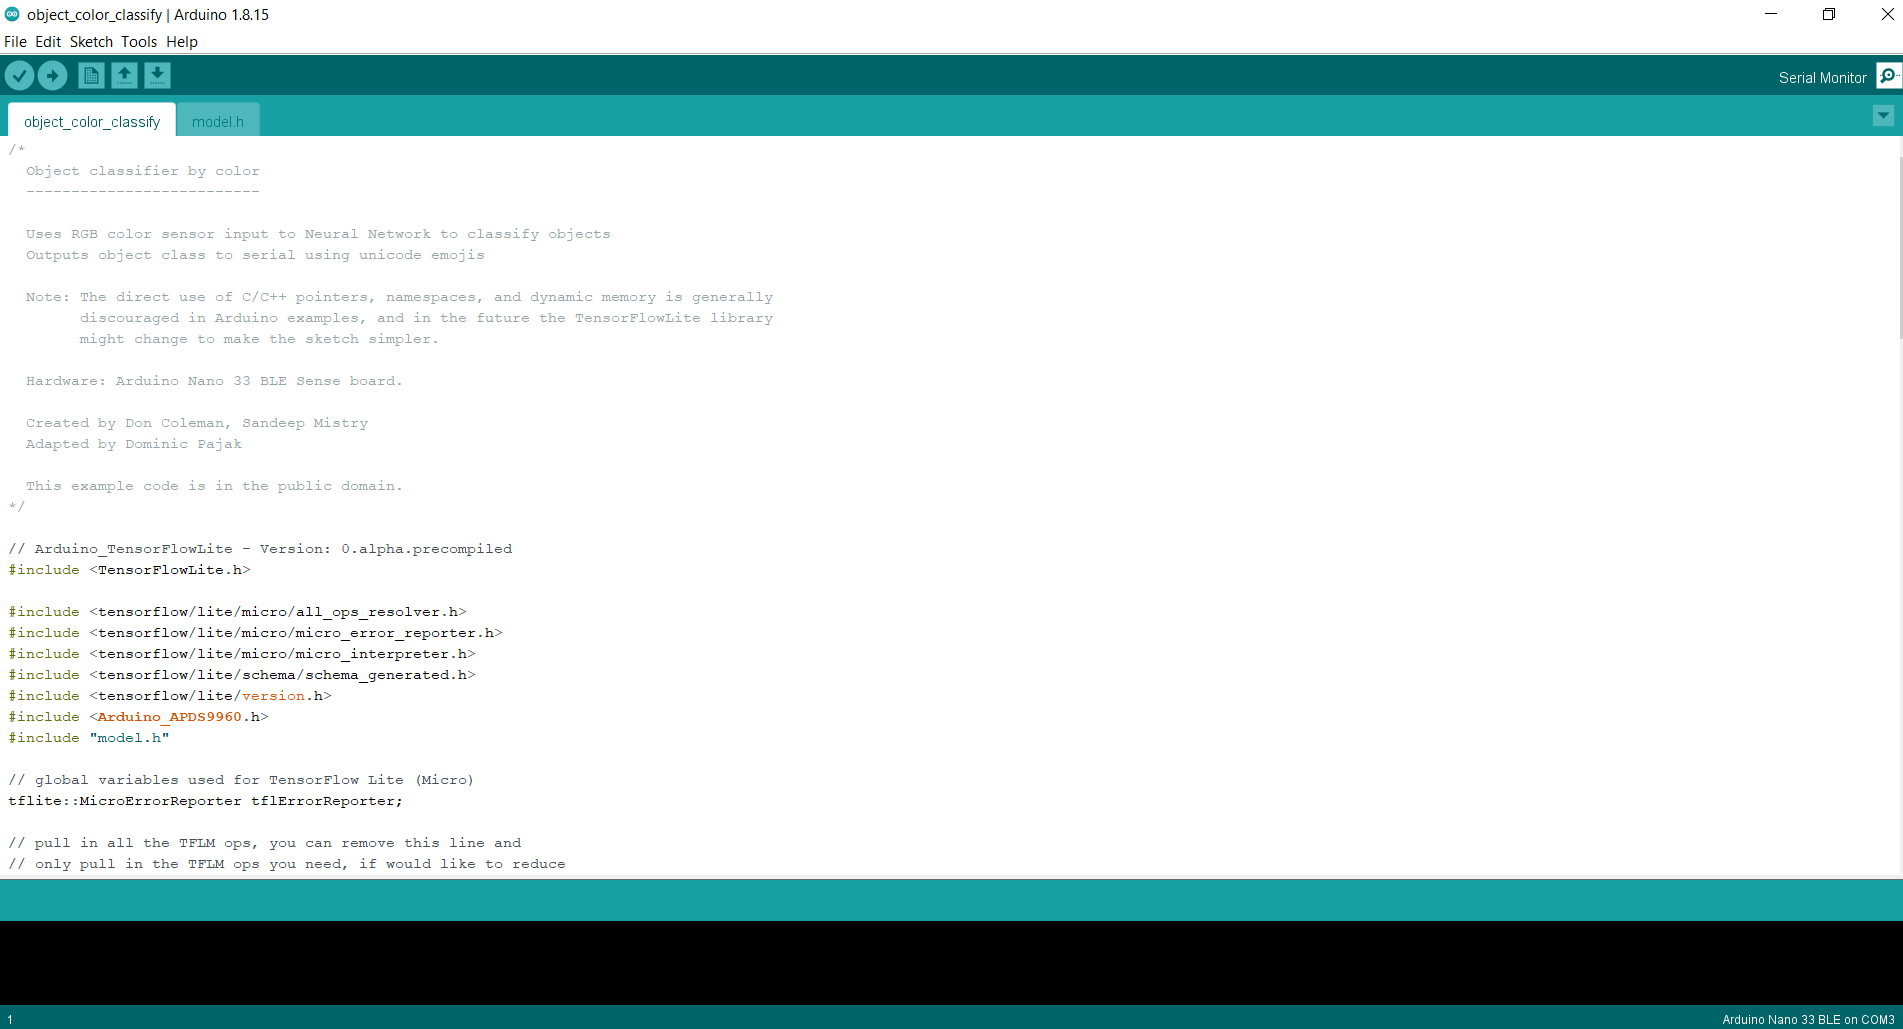
\includegraphics[width=1.0\linewidth]{Images/Nano33BLESense/Serial Monitor}
	\caption{Serial Monitor Icon}
	\label{fig:Serial Monitor}
\end{figure}

The Final results, all the variables, input, sensor values are shown in the serial monitor the (Output Window)  as shown in the figure \ref{fig:Output Window} by clicking the serial monitor button.

\begin{figure}[h]
	\centering
	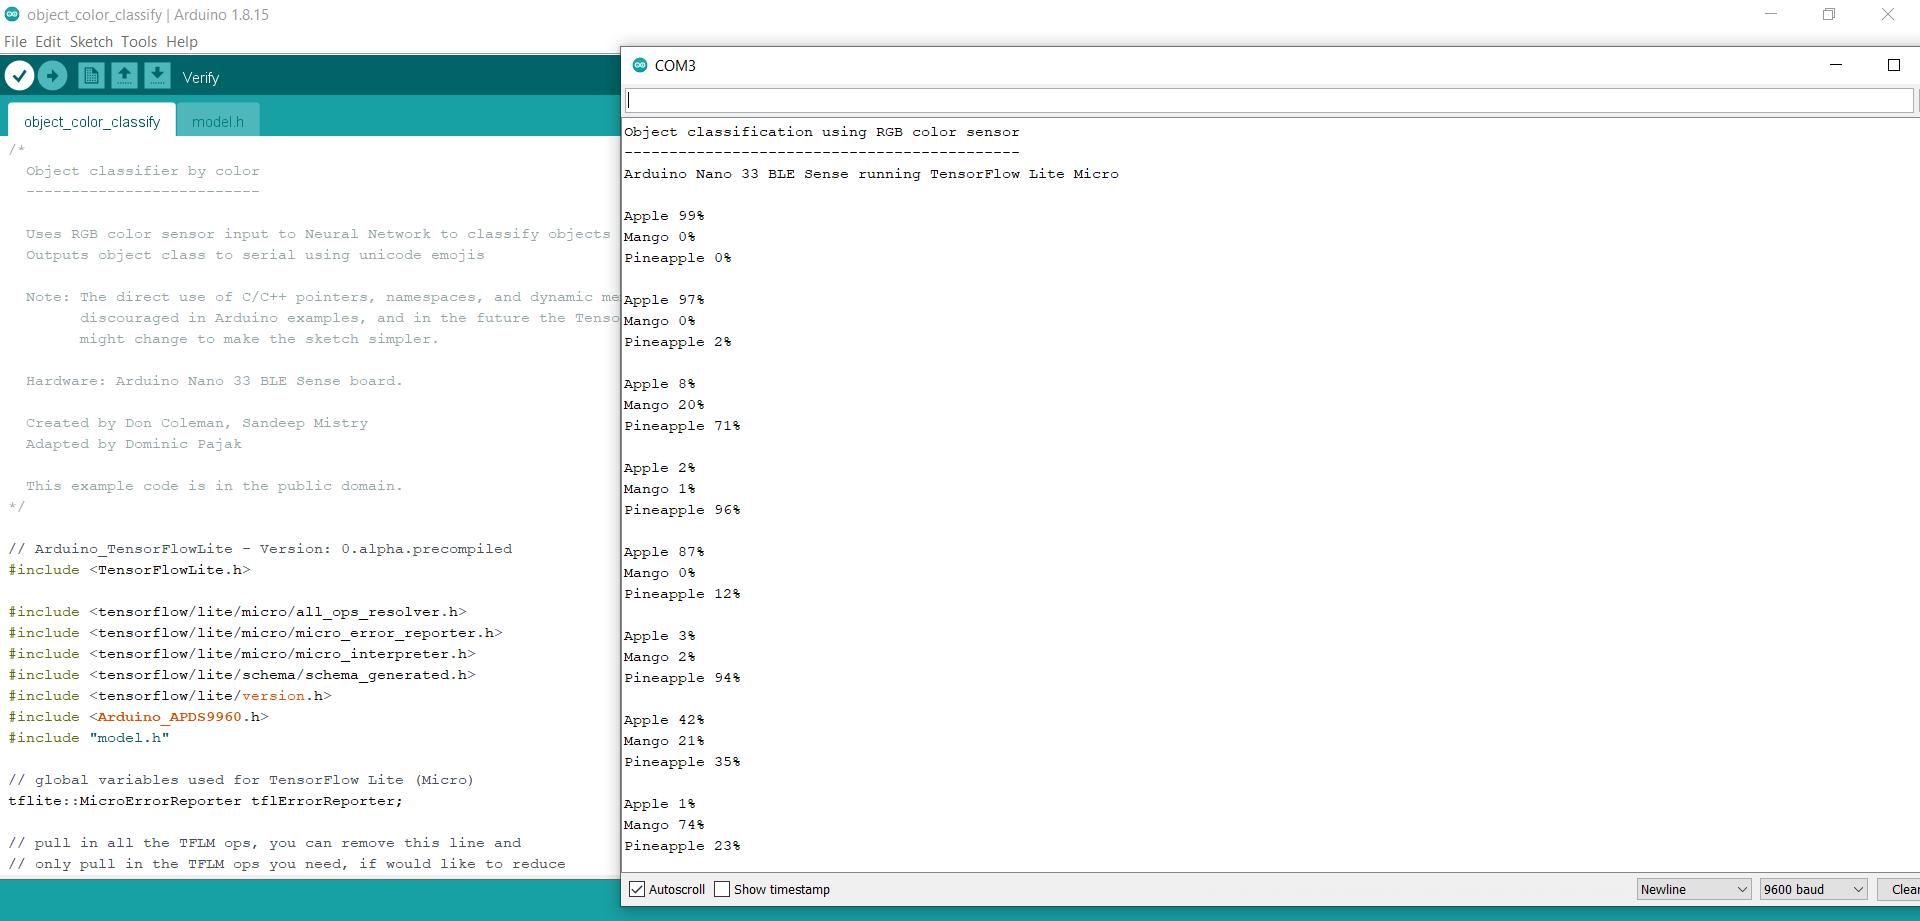
\includegraphics[width=1.0\linewidth]{Images/Nano33BLESense/4}
	\caption{Output Window}
	\label{fig:Output Window}
\end{figure}

%\section{Python on Pycharm}
%
%PyCharm is an integrated development environment (IDE) from the JetBrains company for the Python programming language. This Integrated development environment offers only the python programming environment, which will be usefull later in our project for running some computer vision python module.
%
%
%\subsection{Pycharm Installation}
%
%For getting up to date latest version of pycharm, we need to go \href{https://www.jetbrains.com/pycharm/download/#section=windows}{JetBrains-Link} and install the appropriate version as per our Operating system. 

\section{Python Installation}

Python is commonly used for developing websites and software, task automation, data analysis, and data visualization. Since it's relatively easy to learn, Python has been adopted by many non-programmers such as accountants and Data scientists, for a variety of everyday tasks, like organizing finances. It is an interpreted, object-oriented, high-level programming language with dynamic semantics. \href{https://www.python.org/downloads/}{Python Installation} at the time of writing this report the latest version of python is 3.9.7 release.\ref{Python Installation}

\begin{figure}[h]
	\centering
	\includegraphics[width=1.0\linewidth]{Images/Arduino/python}
	\caption{Python Installation}
	\label{Python Installation}
\end{figure}

\section{Anaconda supporting framework for Jupyter Notebook}

Anaconda is a distribution of the Python and R programming languages for scientific computing (data science, machine learning applications, large-scale data processing, predictive analytics, etc.), that aims to simplify package management and deployment. It is the most popular toolkit for data science environment. It support every package of Machine learning and Artificial Intelligence. The most widely used packages in machine learning are TensorFlow, OpenCV, and MediaPipe. the other supporting libraries include Numpy, Pandas, Matplotlib, Sklearn and many more. For getting up to date documentation and installation guide available at \href{https://www.anaconda.com/products/individual}{Jupyter notebook}. Anaconda support Jupyter notebook web application, it is the most widely used notebook for writing and training the Machine learning models.




%\chapter{Arduino Nano 33 BLE Sense}
%
%\subsection{Hardware}
%\subsection{Software}
%- Datasheet lesen
%- Welcher Sensoren werden benutzt, warum und Welcher format von data ergeben die (IMU) 
%\section{Beschränkungen}
%- Beschränkungen identifizieren : Speicher, Gehäuse, Komplexität, Geschwindigkeit.   
%\section{IMU}
%\subsection{Einleitung}
%\subsection{Hardware}
%- Accelerometers
%- Gyroscope
%- Magnetometers
%\subsection{Software}
%\subsection{Calibration of Sensor Motion}
%\section{Arduino IDE}
%\subsection{Installation}
%\subsection{Configuration}
%\subsection{Tests}
%- Hello World - blink.ino
%-IMU